\documentclass[a4paper,article,14pt]{extarticle}

\usepackage{audiploma}
\usepackage{euscript}
\usepackage{longtable}
\usepackage{makecell}
\usepackage[pdftex]{graphicx}
\usepackage{amsthm,amssymb, amsmath}
\usepackage{textcomp}
\usepackage[style=numeric-comp, sorting = none]{biblatex}
\usepackage{csquotes}

\usepackage{hyperref}
\hypersetup{
    colorlinks=True,
    allcolors=NavyBlue
}
\usepackage[svgnames]{xcolor}

\IfFileExists{pscyr.sty}{\usepackage{pscyr}}{}


%%% Выравнивание и переносы %%%
%% http://tex.stackexchange.com/questions/241343/what-is-the-meaning-of-fussy-sloppy-emergencystretch-tolerance-hbadness
%% http://www.latex-community.org/forum/viewtopic.php?p=70342#p70342
\tolerance 1414
\hbadness 1414
\emergencystretch 1.5em % В случае проблем регулировать в первую очередь
\hfuzz 0.3pt
\vfuzz \hfuzz
%\raggedbottom
%\sloppy                 % Избавляемся от переполнений
\clubpenalty=10000      % Запрещаем разрыв страницы после первой строки абзаца
\widowpenalty=10000     % Запрещаем разрыв страницы после последней строки абзаца
\brokenpenalty=4991     % Ограничение на разрыв страницы, если строка заканчивается переносом

\addbibresource{references.bib}


\begin{document}

% --------------------- Стандарт СПб АУ РАН --------------------------%

\begin{titlepage}

\newgeometry{left=30mm, top=30mm, right=15mm, bottom=30mm, nohead, nofoot}

\vspace{15mm}
\begin{center}
    
\includegraphics[width = \textwidth]{images/autitle.png}
\end{center}

\vspace{0.1mm}

\begin{flushright}
    «\rule{1cm}{0.15mm}» \rule{2cm}{0.15mm} 2021г. \\
    Зав. каф. \\
    Теоретической физики \\
    \rule{25mm}{0.20mm} д.ф.-м.н. С. А. Тарасенко \\
\end{flushright}


\begin{center}

\vspace{9mm}
\textbf{\large ИСПОЛЬЗОВАНИЕ ТУЛИЕВЫХ БОЛОМЕТРОВ В КАЧЕСТВЕ ПЕРЕСПЕКТИВНЫХ ДЕТЕКТОРОВ СОЛНЕЧНЫХ АКСИОНОВ}
\vspace{9mm}

выпускная квалификационная работа бакалавра \\
\vspace{10mm}
Направление 03.03.01 Прикладные математика и физика \\
\vspace{14mm}
\textbf{\large Кузьмичев Артем Михайлович}


\vspace{16mm}

% Научный руководитель
\textbf{Научный руководитель} \hfill \rule{6.5cm}{0.15mm} Е.В. Унжаков \\
\vspace{5mm}
\textbf{Студент} \hfill  \rule{6cm}{0.15mm} А.М. Кузьмичев

\vfill 

{Санкт-Петербург, 2021}
\end{center}
\end{titlepage}
% Возвращаем настройки geometry обратно (то, что объявлено в преамбуле)
\restoregeometry
% Добавляем 1 к счетчику страниц ПОСЛЕ titlepage, чтобы исключить
% влияние titlepage environment
\addtocounter{page}{1}
\tableofcontents
\pagebreak

% Elements and compounds definition
\newcommand{\Tm}{$^{169}$Tm}
\newcommand{\Fe}{$^{57}$Fe}
\newcommand{\Kr}{$^{83}$Kr}

\newcommand{\Pb}{$^{210}$Pb}
\newcommand{\UranA}{$^{235}$U}
\newcommand{\UranB}{$^{238}$U}
\newcommand{\ThA}{$^{228}$Th}
\newcommand{\ThB}{$^{232}$Th}
\newcommand{\RaA}{$^{226}$Ra}
\newcommand{\RaB}{$^{228}$Ra}

\newcommand{\Am}{$^{241}$Am}
\newcommand{\Cs}{$^{137}$Cs}
\newcommand{\Co}{$^{60}$Co}
\newcommand{\K}{$^{40}$K}

\newcommand{\TmAlO}{{Tm$_3$}{Al$_5$}{O$_{12}$}}
\newcommand{\NaTmWO}{NaTm(WO$_4$)$_2$}
\newcommand{\NaTmMoO}{NaTm(MoO$_4$)$_2$}




\specialsection{Введение}
В~настоящее время Стандартная модель является наиболее успешной физической теорией, описывающей элементарные частицы и их взаимодействия.
Тем не менее, существует целый ряд наблюдений и экспериментов, для которых Стандартная модель не даёт адекватных объяснений.
Одним из них является сильная CP-проблема, заключающаяся в~ненаблюдении CP-нарушения в~сильных взаимодействиях.
Так называемый $\theta$-член в лагранжиане квантовой хромодинамики (КХД) отвечает за взаимодействие глюонных полей и имеет следующий вид:

\begin{equation}\label{eq:lagrangian}
    \mathcal{L}_{\text{КХД}} =
    \ldots + \theta \cdot G_{\mu \nu }^a \tilde{G}_a^{\mu \nu}\, .
\end{equation}
Данный член является калибровочно- и лоренц-инвариантным и не нарушает перенормируемости теории, однако в то же время является нечётным относительно P и T преобразований, что должно вести к несохранению CP-симметрии в сильных взаимодействиях в случае $\theta \neq 0$.
Например, теоретически предсказанный дипольный момент нейтрона оказывается равным $\left|{d_n} \right| \sim \theta  \cdot {10^{ - 16}} \text{ е} \cdot \text{см} $ \cite{NDMtheory}.
В то же время, установленный экспериментальный предел $ \left( \left| {{d_n}} \right| < 1.8 \cdot {10^{ - 26}} \text{ е} \cdot \text{см}\left( {90\% \text{ у.д.}} \right) \right)$ \cite{NDMexperiment} позволяет заключить, что $\theta < 10^{-10}$, что делает $\theta$-член очень малым по сравнению с другими слагаемыми лагранжиана КХД.

Решение данной проблемы было предложено в~1977~г.
Роберто Печчеи и Хелен Квинн~\cite{PQ}.
Согласно работе учёных, введение дополнительной киральной симметрии U(1) может скомпенсировать CP-неинвариантное слагаемое в~лагранжиане~КХД за~счёт спонтанного нарушения этой симметрии на~некотором энергетическом масштабе $f_A$.
В~результате такого нарушения, как показали чуть позже Стивен Вайнберг~\cite{Weinberg} и Фрэнк Вильчек~\cite{Wilczek} за~счёт механизма Намбу-Голдстоуна возникает новая псевдоскалярная нейтральная частица.
Название <<аксион>> дано Ф.~Вильчеком по~марке стирального порошка, так как аксион должен <<очищать>> КХД от~сильной CP-проблемы; а~также из-за связи с~осевым (англ.~\textit{axial}) током.

В~первоначальной стандартной" модели аксиона, также называемой моделью PQWW-аксиона (Peccei-Quinn-Weinberg-Wilczek) масштаб нарушения симметрии совпадал с масштабом электрослабого взаимодействия:
$f_A \approx \frac{1}{(\sqrt{2} G_F)^{1/2}} \approx 250$~ГэВ.
Тем самым, нижняя граница взаимодействия с~веществом оказалась предопределена теорией и необнаружение его в~проведённых экспериментах по поиску аксиона на реакторах~\cite{ReactorExperiment1,ReactorExperiment2} и на ускорителях~\cite{AcceleratorExperiment1,AcceleratorExperiment2} надёжно исключили возможность существования стандартного аксиона.

Два класса теоретических моделей так называемого <<невидимого>> аксиона, адронный аксион и GUT-аксион, так или иначе подавляют его взаимодействие c~обычным веществом: фотонами~($g_{A\gamma}$), лептонами~($g_{Ae}$) и нуклонами~($g_{AN}$), в то же время сохраняя его в~виде, необходимом для решения сильной CP-проблемы.
Масса аксиона и его константы связи оказываются обратно пропорциональны масштабу $f_A$, который, в~отличие от~модели <<стандартного>> аксиона, не фиксируется, а может быть произвольным, вплоть до~планковских значений $~10^9 \text{ ГэВ}$, подавляя тем самым его взаимодействия.

Результаты современных экспериментов интерпретируются преимущественно в рамках этих двух наиболее популярных моделей.
Основные экспериментальные усилия сосредоточены на поиске аксиона с массой в диапазоне $10^{-6} \div 10^{-2}$~эВ.
Этот диапазон свободен от~астрофизических и космологических ограничений, кроме того, реликтовые аксионы с~такой массой считаются наиболее вероятными кандидатами на роль частиц, образующих темную материю.
Имеются и другие предпосылки к активным поискам новой частицы.
Существование аксионов или ALP (аксионоподобных частиц, от англ. \textit{Axion-Like Particle}) могло бы объяснить слишком быстрое охлаждение ряда классов звезд~\cite{whitedwarfs}, а также аномальную прозрачность Вселенной для гамма-квантов с~энергией порядка $1$~ТэВ~\cite{transparency,transparency_axion}.

Целью настоящей работы являлся расчёт чувствительности планируемого эксперимента по поиску резонансного поглощения ядром {\Tm} солнечных аксионов с энергией $E = 8.41$~кэВ.
Опираясь на измеренные экспериментальные спектры сырья для болометрического детектора, а также интенсивность фоновых событий подземной низкофоновой установки, были определены необходимые параметры симулируемых процессов (прежде всего, рождения частиц) в модели эксперимента в Geant4.
Полученный спектр симуляции позволяет установить предел на~константы связи аксиона с~веществом, при котором связанные с~ним события в~пике c~энергией $E = 8.41$~кэВ можно будет на~достаточном уровне достоверности выделить на~фоне остальных событий, зарегистрированных болометром.

\pagebreak
\section{Обзор теории и экспериментов по поиску аксиона}

\subsection{Появление в теории, PQWW-аксион}
Первое появление аксиона в~теории связано c~проблемой ненаблюдения CP-нарушения в~сильных взаимодействиях.
В~1977 году Роберто Печчеи и Хелен Квинн~\cite{PQ}, находясь в~поисках решения данной проблемы, предложили ввести дополнительную киральную симметрию. Спонтанное нарушение симметрии Печчеи-Квинн $U{\left( 1 \right)_{PQ}}$ компенсирует $CP$-неинвариантное слагаемое в~лагранжиане КХД.
Как показали Стивен Вайнберг и Фрэнк Вилчек~\cite{Weinberg,Wilczek}, в~результате такого нарушения за~счёт механизма Намбу--Голдстоуна возникает новая псевдоскалярная нейтральная частица.
Новое аксионное поле $\phi_A$ вводится в~лагранжиан заменой  $\theta \mapsto \theta - \phi_A / f_A$:
\begin{equation}
    \mathcal{L}_{\text{QCD}} =
    \ldots + \left( \theta - \phi_A / f_A \right) \,
    G_{\mu \nu }^a \tilde{G}_a^{\mu \nu} \, .
\end{equation}

В~первоначальной <<стандартной>> модели аксиона масштаб нарушения симметрии $f_A$ совпадал с~масштабом электрослабого взаимодействия:
\begin{equation}
    f_A \approx \frac{1}{(\sqrt{2} G_F)^{1/2}} \approx 250 \text{\ ГэВ} \, ,
\end{equation}
в то время как ожидаемая масса аксиона в данной теории получалась равной:
\begin{equation}\label{mPQWW}
    {m_A} \approx
    \left(
    {25 \text{\ кэВ}}
    \right)
    N \left(
    {X + \frac{1}{X}}
    \right) \, ,
\end{equation}
где $N$ -- число поколений кварков, $X$ -- неизвестный параметр, вычисляемый как отношение вакуумных средних значений хиггсовских полей.
Исходя из~$N = 3$ и неравенства о~средних $X + \frac{1}{X} \geqslant 2$ можно заключить, что масса должна превышать $150$~кэВ.

Реакторные эксперименты и эксперименты с~искусственными источниками~\cite{ReactorExperiment1,ReactorExperiment2} пытались обнаружить аксион по~наиболее вероятной моде распада $A \rightarrow 2\gamma$.
В~ускорительных экспериментах~\cite{AcceleratorExperiment1,AcceleratorExperiment2} предпринимались попытки обнаружить распады каонов ($K^+ \rightarrow \pi^+ + A$) и пионов ($\pi^+ \rightarrow e^+ + \nu + A$), тяжелых кваркониев ($J/\Psi \rightarrow A + \gamma$ и $\Upsilon \rightarrow A + \gamma $), а также распады самого аксиона на два $\gamma$-кванта или на электрон-позитронную пару после рождения его в реакции $p(e) + N \rightarrow A + X $.
Необнаружение аксионов в проведённых экспериментах надёжно исключили возможность существования PQWW-аксиона.

\subsection{<<Невидимый>> аксион}
Два класса теоретических моделей так называемого <<невидимого>> аксиона, так или иначе, подавляют его взаимодействие c~обычным веществом, тем не менее сохраняя его в виде, необходимом для решения сильной CP-проблемы:
\begin{enumerate}
    \item Адронный или KSVZ (Kim, Shifman, Vainshtein, Zakharov) аксион~\cite{K,SVZ} (постулируется наличие дополнительного тяжёлого кварка)
    \item GUT или DFSZ (Dine, Fischler, Srednicki, Zhitnitskii) аксион~\cite{DFS,Z} (вводятся добавочные хиггсовские поля)
\end{enumerate}
Масса аксиона и его константы связи оказываются обратно пропорциональны энергетическому масштабу нарушения симметрии $f_A$, который, в~отличие от~модели <<стандартного>> аксиона, не фиксируется, а может быть произвольным, вплоть до~планковских значений $~10^9$~ГэВ, подавляя тем самым взаимодействие с~обычным веществом:

\begin{equation}\label{mA}
    m_A \approx
    \frac{f_\pi m_\pi}{f_A}
    \left(
    \frac{z}{(1 + z +w) (1 + z)}
    \right)^{\frac{1}{2}} \approx
    \frac{6.0 \times 10^6}{f_A \text{\ (ГэВ})}
\end{equation}
где $z$ и $w$ -- отношения масс легких кварков ($z = m_u/m_d \approx 0.59$, $w = m_u/m_s \approx 0.029$), a $m_{\pi} \approx 135$~МэВ и $f_{\pi} \approx 93$~МэВ -- соответственно, масса и распадная константа пиона.

Экспериментальное закрытие гипотезы PQWW-аксиона указывает на то, что масштаб нарушения симметрии превышает масштаб электрослабого взаимодействия.
С~учётом верхнего предела в~виде планковской массы получаем $250 \text{ ГэВ} \approx f_{\text{PQWW}} < f_A < m_{\mathrm{P}} \approx 10^{19} \text{ ГэВ} $, откуда следует, что диапазон возможных масс новой частицы $10^{-12} \text{\ эВ} \lessapprox m_A \lessapprox 100 \text{\ кэВ}$.

\subsection{Астрофизические ограничения}
Имеется целый ряд астрофизических и космологических соображений~\cite{turner1990windows,Raffelt:1995ym,raffelt1990astrophysical}, позволяющих ввести ограничения на~параметры новой частицы.
Так, данные по~вспышке сверхновой SN1987A позволили получить верхний предел на~массу $m_A < 10^{-3}$~эВ для DFSZ аксиона.
В~отличие от~DFSZ-аксиона, адронный аксион не имеет взаимодействия с~лептонами в~древесном порядке, поэтому ограничения на~его массу в~модели слабее.

В целом из астрофизических данных следует, что аксион должен иметь массу в диапазоне $10^{-5} \div 10^{-3}$~эВ.
Для KSVZ-аксиона существует дополнительное окно диапазоне $10^{-1} \div 10 \text{ эВ}$.
Следует отметить, что данные ограничения получены в моделях предполагающих строгую связь $f_A \cdot m_A \approx f_{\pi} \cdot m_{\pi}$.
В моделях, включающих взаимодействие нашего мира с~зеркальным~\cite{berezhiani2001strong}, данное соотношение не выполняется, что приводит к~существованию неисключенного никакими имеющимися наблюдательными данными окна для аксиона около энергии $1$~МэВ.


\pagebreak
\section{Резонансное поглощение солнечных аксионов}

\subsection{Поток и энергетический спектр солнечных аксионов}
Существование новой частицы должно приводить к тому что звёзды, в том числе Солнце, должны являться мощным источником аксионов, рождаемых в следующих процессах:
\begin{enumerate}
    \item Обратный эффект Примакова для аксиона ($g_{A\gamma}$)
    \item Аксионное тормозное излучение ($g_{Ae}$)
    \item Комптоновское рассеяние аксиона ($g_{Ae}$)
    \item Атомные переходы магнитного типа ($g_{Ae}$)
    \item Ядерные реакции ($g_{AN}$)
    \item Тепловое возбуждение ядер ($g_{AN}$)
\end{enumerate}
В~ряде предыдущих работ по~поиску резонансного поглощения солнечных аксионов~\cite{prevax57Fe,prevaxLi7,83Kr} механизмы, связанные с~возбуждением ядерных уровней за~счёт высокой температуры, предполагались основным источником аксионов ввиду наличия данных элементов на~Солнце.
Современные солнечные модели не дают конкретных прогнозов о~содержании тулия на~Солнце, в~связи с~чем в~настоящей работе уделяется внимание другим процессам рождения.

Обратный эффект Примакова для аксиона назван по~аналогии с~конверсией пиона в~фотон в~поле ядра, и обеспечивает конверсию фотонов в~аксионы в~электромагнитном поле плазмы.
Лагранжиан, описывающий взаимодействие аксионного поля $\phi_A$ с~электромагнитным полем, которое задаётся тензором $F^{\alpha \beta}$:
\begin{equation}
    \mathcal{L} =
    g_{A\gamma}\, \varphi_A\, F_{\alpha\beta} \tilde{F}^{\alpha\beta} =
    g_{A\gamma}\, \varphi_A\,\vec{B} \cdot \vec{E}\, .
\end{equation}
Соответствующая данному взаимодействию константа связи $g_{A\gamma}$ в моделях <<невидимого>> аксиона равна:
\begin{equation}\label{gAy}
    g_{A\gamma} =
    \frac{\alpha}{2 \pi {f_A}}
    \left[
        \frac{E}{N} - \frac{2}{3} \frac{(4 + z)}{(1 + z)}
        \right] =
    \frac{\alpha}{2 \pi {f_A}} C_{A\gamma\gamma}\, ,
\end{equation}
где $\alpha = 1/137 $ -- постоянная тонкой структуры; $z$ и $w$ -- отношения масс легких кварков ($z = m_u/m_d \approx 0.59$, $w = m_u/m_s \approx 0.029$); остальные параметры являются модельно зависимыми:
\begin{table}[h]
    \centering
    \begin{tabular}{|l|c|c|}
        \hline
        Теоретическая модель                                    & $E/N$ & $C_{A\gamma\gamma}$ \\
        \hline
        \hline
        GUT-аксион (DFSZ)                                       & $8/3$ & $0.74$              \\
        \hline
        Адронный аксион (KSVZ)                                  & $0$   & $-1.92$             \\
        \hline
        Альтернативная модель адронного аксиона~\cite{hadronic2} & $2$   & $0$                 \\
        \hline
    \end{tabular}
    \caption{Константа связи с фотоном в разных моделях аксиона}\label{tab:gay}
\end{table}\newline
Аксионы, рождённые при конверсии фотонов Солнца и достигнувшие поверхности земли имеют следующий энергетический спектр~\cite{solarflux1,solarflux2,solarflux3}:
\begin{equation}
    \frac{d \Phi_A}{d E_A} =
    \left(
    \frac{g_{A\gamma}}{10^{-10} \text{\ ГэВ}}
    \right)^2
    \frac{\Phi_0}{E_0}\,
    \frac{(E_A / E_0)^3}{\exp(E_A / E_0) - 1}
    \left[
        \text{см}^{-2} \cdot \text{с}^{-1} \cdot \text{кэВ}^{-1}
        \right]
\end{equation}
где ${E_0} = kT = 1.103 \text{\ кэВ}$ -- температура плазмы Солнца в энергетических единицах, ${{\Phi _0}} = 5.95 \cdot 10^{14} \text{ см} ^{-2} \text{ с} ^{-1}$ -- \emph{???}.

Ожидаемый поток аксионов за~счёт взаимодействий $g_{Ae}$, вычисляется с~использованием сечений для комптоновских процессов~\cite{pospelov2008bosonic,gondolo2009solar} и тормозного излучения~\cite{brem}, данных стандартной солнечной модели о~плотности электронного газа, распределении температуры и концентрациях различных элементов~\cite{kekez2009search,derbin2011constraints}. Учёт образования аксионов с~помощью процессов атомной рекомбинации произведён в~работе~\cite{redondo2013solar}.
Формы спектров солнечных аксионов для перечисленных процессов образования приведены на рис.~\ref{fig:flux}.
\begin{figure}[t]
    \centering
    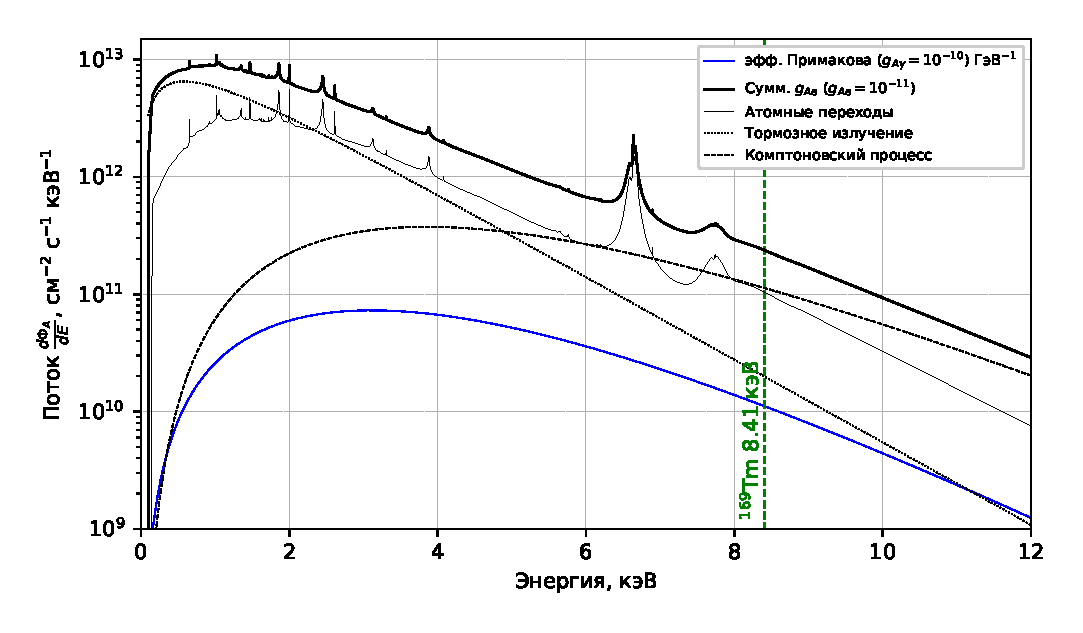
\includegraphics[width = .9\textwidth]{images/flux_solar_ru.eps}
    \caption{Форма спектров солнечных аксионов. Расчёт выполнен для номинальных значений $g_{A\gamma} = 10^{-10}$~ГэВ$^{-1}$ и $g_{Ae} = 10^{-11}$ при $m_A = 0$.}\label{fig:flux}
\end{figure}
Воспользовавшись зависимостями \eqref{mA} и \eqref{gAy}, можно получить полный поток аксионов от данного процесса в терминах $m_A$:
\begin{equation}
    \Phi_A =
    \int\limits_0^{+\infty} \frac{d\Phi_A}{dE_A} d{E_A} =
    7.44 \times 10^{11}
    \left(
    \frac{m_A}{1 \text{\ эВ}}
    \right)
    \left[
        \text{см}^{-2} \cdot \text{с}^{-1}
        \right]
\end{equation}

Предпринимались попытки обнаружить данные аксионы при конверсии аксиона обратно в~фотон в~лабораторных магнитных полях (BNL~\cite{lazarus1992search}, Tokio axion helioscope~\cite{moriyama1998direct,inoue2002search}, CAST -- CERN Axion Solar Telescope~\cite{beltran2005search}).
Кроме того, другой возможный механизм поиска --- когерентная конверсия аксиона в~фотон в~поле кристалла~\cite{paschos1994proposal} --- лег в~основу экспериментов с~германиевыми детекторами SOLAX~\cite{avignone1998first, avignone1999solar} и COSME~\cite{scopel1998theoretical,morales2002particle}, а также DAMA \cite{bernabei2001search} --- c детектором на основе кристалла NaI.
Установленные верхние пределы на~константу связи варьируются в~диапазоне $g_{A \gamma} \leqslant 10^{-10} \div 10^{-8}$.

\subsection{Резонансное поглощение аксиона в ядерных переходах магнитного типа}
Аксион способен испытывать резонансное поглощение атомным ядром в~переходах магнитного типа, так как является псевдоскалярной частицей.
Релаксация возбужденных ядер приводит к~образованию $\gamma$-квантов, а также конверсионных и Оже-электронов, которые могут быть зарегистрированы обычными средствами.
Изотопы {\Fe}, {\Kr} и {\Tm} обладают подходящими низколежащими ядерными переходами для поиска аксиона данным методом.

В~Петербургском институте ядерной физики активно ведутся эксперименты по~поиску резонансного поглощения солнечных аксионов~\cite{Derbin2005,Derbin2007,Derbin2009,muratova2015searches,newlimits_tm}.
Первые эксперименты были выполнены по~схеме <<мишень-детектор>> c~нуклидами {\Fe} и {\Tm} имеющих энергию первого возбуждённого уровня $14.4$~кэВ и $8.41$~кэВ, соответственно.
Мишень устанавливалась непосредственно над полупроводниковым Si(Li) детектором.
Сама установка находилась на поверхности земли, но была снабжена активной защитой, для защиты от космогенных компонент фона.
В результате проведённых измерений были получены ограничения на аксион-нуклонную константу связи:
\begin{equation}
    ^{57}\text{Fe:\ }
    \left| {g_{AN}^3 + g_{AN}^0} \right| \leqslant
    3.12 \times 10^{-6};\quad m_A \leqslant 151 \text{\ эВ}\, ,
\end{equation}
и произведение аксион-фотонной и аксион-нуклонной констант:
\begin{equation}
    ^{169}\text{Tm:\ }
    g_{A\gamma} \left| {g_{AN}^3 + g_{AN}^0} \right| \leqslant
    9.2 \times {10^{ - 13}};\quad m_A \leqslant 191 \text{\ эВ}\, .
\end{equation}

Следующим шагом было создание низкофоновой установки в~сотрудничестве с~Баксанской Нейтринной Обсерваторией (БНО) на~базе газового пропорционального счётчика~\cite{83Kr}.
Глубокое расположение ($4800$~м водного эквивалента) обеспечило снижение космогенного фона и увеличило чувствительности эксперимента.
В установке был использован газообразный криптон, обогащённый изотопом {\Kr}. Предыдущие ограничения на аксион-нуклонную константу были улучшены приблизительно на порядок и составили~\cite{Derbin_2017_Kr}:
\begin{equation}
    ^{83}\text{Kr}:
    \left| {g_{AN}^3 - g_{AN}^0} \right| \leqslant
    8.4 \cdot {10^{ - 7}};\quad {m_A} \leqslant 65 \text{\ эВ}
\end{equation}

\subsection{Резонансное поглощение аксионов ядрами {\Tm}}

Рассмотрим подробнее процесс резонансного поглощения аксионов ядром тулия, с последующим излучением гамма-кванта: $A + {}^{169}\mathrm{Tm} \rightarrow {}^{169}\mathrm{Tm}^{*} \rightarrow {}^{169}\mathrm{Tm} + \gamma$.
Схема уровней нуклида {\Tm} показана на~рис.~\ref{tmlvls}.
Первый возбуждённый уровень ($3/2^+$) имеет энергию $E = 8.41 \text{\ кэВ}$, c  примесью вероятности перехода E2-типа $\delta = 0.033$.
С учётом относительно высокого коэффициента внутренней конверсии ($\frac{e}{\gamma} = 285$~\cite{lederer1978table}) вероятность излучения гамма-кванта при разрядке данного уровня составит $\eta = \frac{1}{1 + e/\gamma} \approx 3.5 \cdot 10^{-3}$.
\begin{figure}[t]
    \centering
    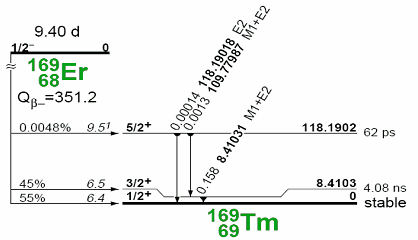
\includegraphics[width = 0.75 \textwidth]{images/Tmlevels.png}
    \caption{Схема уровней ядра {\Tm}~\cite{lederer1978table}}\label{tmlvls}
\end{figure}

Сечение резонансного поглощения аксионов можно получить из выражения для сечения поглощения гамма-квантов, с учётом отношения вероятностей излучения аксиона и фотона $\frac{\omega_A}{\omega _{\gamma}}$ в данном переходе \cite{donnelly1978axions}:
\begin{equation}\label{eq:sech}
    \sigma(E_A) =
    \pi \sigma_{0_\gamma} \Gamma
    \left(
    \frac{\omega _A}{\omega _\gamma}
    \right)
\end{equation}
\begin{equation}\label{eq:wAwy}
    \frac{\omega_A}{\omega_\gamma} =
    \frac{1}{2 \pi \alpha (1 + \delta^2)}\,
    \frac{g_{AN}^3 \beta + g_{AN}^0}{(\mu_0 - 0.5)\beta + \mu_3 - \eta}
    \left(
    {\frac{{{p_A}}}{{{p _\gamma }}}}
    \right)^3
\end{equation}
где  $\sigma_{0\gamma}$ -- максимальное сечение резонансного поглощения гамма-квантов (экспериментально определённое значение для {\Tm} составляет $\sigma_{0\gamma} = 2.56 \times 10^{19} \text{ см}^2$).
Из времени жизни первого возбуждённого уровня $\tau = 5.89 \text{ нс}$ можно получить собственную ширину уровня $\Gamma = 1.13 \cdot 10^{-7}$.
Далее, $p_A$ и $p_{\gamma}$ -- импульсы аксиона и фотона, соответственно; $\alpha = 1/137$ -- постоянная тонкой структуры, $\mu_0 = \mu_p + \mu_n \approx 0.88$ и $\mu_3 = \mu_p - \mu_n \approx 4.71$ -- изоскалярный и изовекторный ядерные магнитные моменты; параметры $\beta$ и $\eta$ задаются ядерными матричными элементами:
\begin{equation}
    \eta =
    - \frac{
    \left\langle
    J_f
    \left|
    \sum\limits_{i = 1}^A {l(i){\tau_3}(i)}
    \right|
    J_i
    \right\rangle
    }
    {
    \left\langle
    J_f
    \left|
    \sum\limits_{i = 1}^A {\sigma (i){\tau _3}(i)}
    \right|
    J_i
    \right\rangle
    }\, ,
\end{equation}
\begin{equation}
    \beta =
    - \frac{
        \left\langle
        J_f
        \left|
        \sum\limits_{i = 1}^A \sigma (i)
        \right|
        J_i
        \right\rangle
    }
    {
        \left\langle
        J_f
        \left|
        \sum\limits_{i = 1}^A \sigma (i){\tau _3}(i)
        \right|
        J_i
        \right\rangle
    }\, ,
\end{equation}
и в случае ядра {\Tm}, имеющего нечётное число нуклонов и неспаренный протон, составляют $\beta \approx 1$ и $\eta \approx 0.5$.

Скорость поглощения солнечных аксионов $R_A$ одним ядром {\Tm} в единицу времени выражается как $R_A = \sigma(E_A)\,\left.\frac{d\Phi_A}{dE_A} \right|_{E_A = 8.14 \text{\ кэВ}}$.
Тогда, используя выражения для сечения~(\ref{eq:sech}), отношения вероятностей~(\ref{eq:wAwy}), констант взаимодействия~(\ref{}) и массы аксиона, мы можем записать $R_A$:
\begin{itemize}
    \item[•] в терминах констант связи
          \begin{align}\label{RAg1}
               & R_A =
              C_{Ax}\, g_{Ax}^2\,(g_{AN}^0 + g_{AN}^3)^2
              \left(\frac{p_A}{p_\gamma}\right)^3 \\
               & C_{A\gamma } = 104\, ,\quad
              C_{Ae} = 2.76 \times {10^5}\, ;\nonumber
          \end{align}
    \item[•] в терминах произведения констант связи и массы
          \begin{align}\label{RAg}
               & {R_A} =
              C'_{Ax}\, g_{Ax}^2\, m_A^2
              \left(\frac{p_A}{p_\gamma}\right)^3             \\
               & C_{A\gamma } = 4.08 \times 10^{-13}\, ,\quad
              C_{Ae} = 1.03 \times {10^{-9}}\, ;\nonumber
          \end{align}
    \item[•] в терминах массы аксиона
          \begin{align}\label{RAm}
               & R_A =
              C''_{Ax} m_A^4
              \left(\frac{p_A}{p_\gamma}\right)^3               \\
               & C''_{A\gamma } = 6.64 \times 10^{-32}\, ,\quad
              C''_{Ae} = 8.08 \cdot 10^{-31}\, .\nonumber
          \end{align}
\end{itemize}
В~приведённых формулах $m_A$ масса аксиона выражена в~единицах эВ.
Константы $C_{Ax}$, а также их пересчитанные версии $C'_{Ax }$ и $C''_{Ax }$, зависят от аксионной модели, мишени и др. параметров и были вычислены для ядер {\Tm} в~работах~\cite{Derbin2009,redondo2013solar}.

\subsection{Использование тулиевых  болометров}
Работы~\cite{Derbin2007,Derbin2009,derbin2011constraints} по~поиску аксиона с~помощью реакции резонансного поглощения ядром {\Tm} были выполнены в схеме мишень-детектор. Наилучшие полученные ограничения:
\begin{align}
     & g_{Ae}\,\left| g_{AN}^3 + g_{AN}^0 \right| \leqslant
    2.1 \times 10^{-14}\, ,                                 \\
     & g_{Ae} \cdot {m_A} \leqslant
    3.1 \times 10^{-7} \text{ эВ}\, .
\end{align}

Внесение вещества мишени в~рабочий объём детектора позволяет существенно увеличить чувствительность эксперимента.
Нивелируется самопоглощение гамма-квантов веществом мишени.
Низколежащие ядерные уровни имеют значительные коэффициенты внутренней конверсии ($\approx 10^{-2}$), поэтому практически вся энергия рассеивается в~детекторе.
При этом необходимо достаточно сильное подавление фонов, так как тулий имеет ряд характеристических рентгеновских линий, близких к~энергии $8.41$~кэВ~\cite{Derbin2009}.

Первые попытки задействовать тулийсодержащие кристаллы {\NaTmWO} и {\NaTmMoO} в~экспериментах по~поиску аксиона были изложены в~работе~\cite{tm_first}.
Использование охлаждённого до $10$~мК кристалла тулиевого граната ({\TmAlO}) в~качестве болометрического криогенного детектора изучено в~работе~\cite{test_bolometric_tm}.
Проведённые измерения подтвердили принципиальную возможность его использования в экспериментах по поиску, тем не менее, указали на ряд сложностей, которые необходимо преодолеть.
В частности, радиационная чистота сырья должна быть повышена для уменьшения влияния естественной радиоактивности на низкофоновый эксперимент; разрешение детектора также требует оптимизации.
Следует заметить, что, хотя ряд российских ученых участвуют в международных экспериментах по поиску $2\beta$-распада и темной материи с использованием криогенных болометров, для российских институтов методика съема сигнала с больших кристаллов, охлажденных до $10$~мК, является принципиально новой.

Недавняя работа~\cite{newlimits_tm} реализовала описанный эксперимент для тулиевого болометра с датчиком края перехода (Transition Edge Sensor), напыленным непосредственно на поверхность кристалла.
Эффективная экспозиция составила $19.2$~$\text{г} \cdot \text{день}$. Полученные ограничения:
\begin{align}
     & g_{A\gamma} \left| g_{AN}^3 + g_{AN}^0 \right| \leqslant
    1.44 \times 10^{-14} \text{\ ГэВ}^{-1}\, ,                  \\
     & g_{A\gamma } \cdot m_A \leqslant
    2.31 \times 10^{-7}\, ;\nonumber
\end{align}
\begin{align}
     & g_{Ae} \left| g_{AN}^3 + g_{AN}^0 \right| \leqslant
    2.81 \times 10^{-16}\, ,                               \\
     & g_{Ae} \cdot {m_A} \leqslant
    4.59 \times 10^{-9} \text{\ эВ}\, .\nonumber
\end{align}
Здесь масса аксиона выражена в единицах эВ, $g_{A\gamma }$ --- в $\text{ ГэВ}^{-1}$, а константы $g_{Ae }$, $g_{AN}^0$ и  $g_{AN}^3$ --- безразмерны.
Данные ограничения значительно улучшают результаты с~тулием в~схеме мишень-детектор~\cite{Derbin2009}, тем не менее, всё ещё уступают результатам эксперимента с~{\Kr}~\cite{Derbin_2017_Kr}.
\begin{figure}[t]
    \centering
    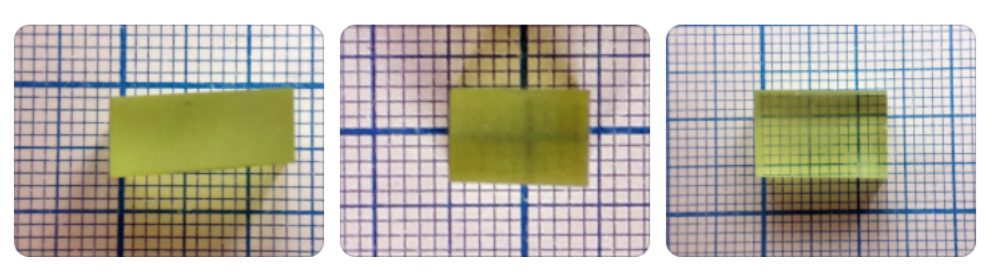
\includegraphics[width=.9\textwidth]{images/Crystals.png}
    \caption{Образцы кристаллов тулий-содержащего граната {\TmAlO}.}\label{fig:crystals}
\end{figure}

В~настоящее время идёт процесс подготовки к~эксперименту в~криогенной установке с~хорошими низкофоновыми характеристиками.
Измерены спектры естественной радиоактивности сырья, выращена новая партия кристаллов тулиевого граната~(\ref{fig:crystals}).
Симуляция данного эксперимента с целью расчёта его чувствительности и является задачей данной работы.


\pagebreak
\section{Оценка параметров симуляции}

\subsection{Эффективность регистрации HPGe детектора}
\begin{figure}[h]
    \centering
    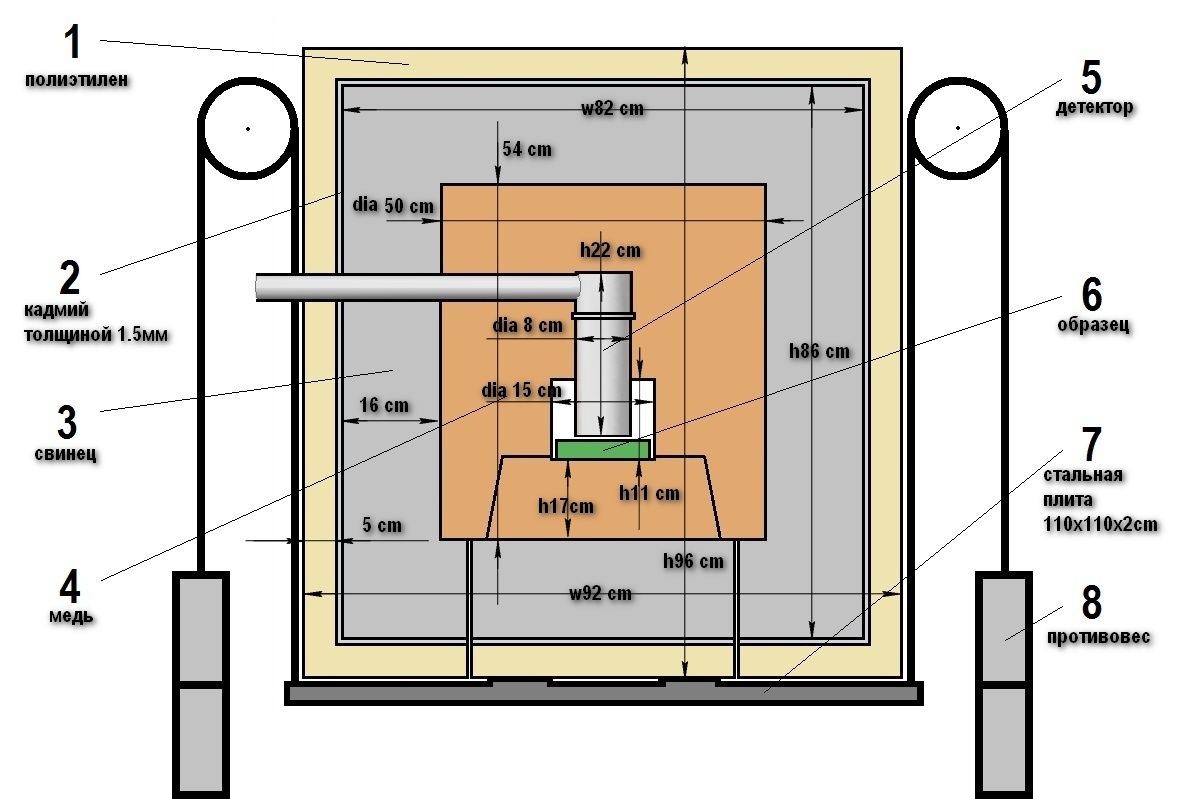
\includegraphics[width=.9\textwidth]{images/farPPD_size.jpg}
    \caption{Геометрические параметры установки farPPD.}\label{fig:geom}
\end{figure}
Для исследования чистоты сырья, используемого для изготовления тулиевого болометра, были произведены измерения на подземной установке с HPGe-детектором в Баксанской Нейтринной Обсерватории (БНО).
Данная установка была промоделирована в Geant4 с целью получения зависимости эффективности регистрации детектора от энергии гамма-частицы, выпускаемой в объёме условного образца.
Схема установки изображена на рис.~\ref{fig:geom}.
Визуализация модели в Geant 4 представлена на рис.~\ref{fig:vis}~и~\ref{fig:tracks}.
\begin{figure}[t]
    \centering
    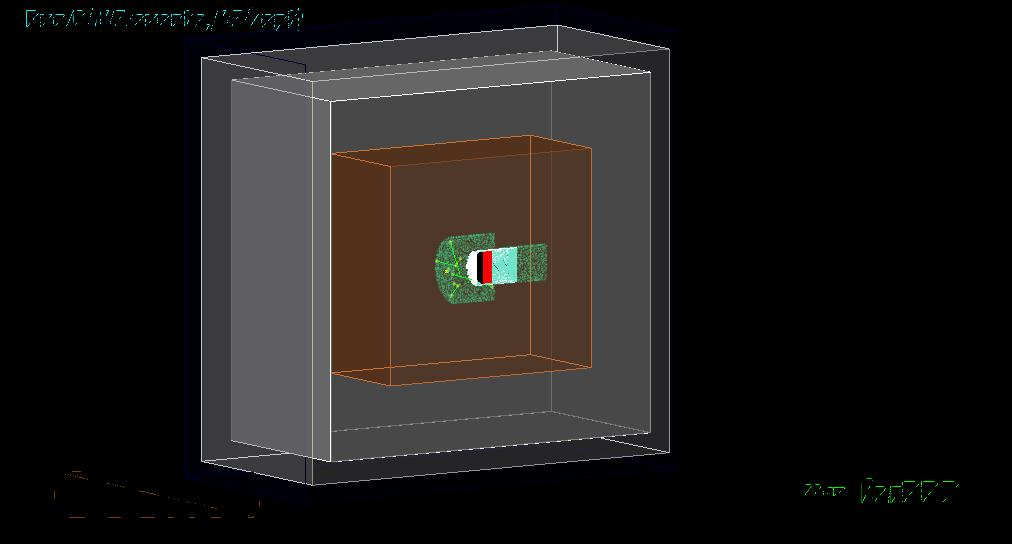
\includegraphics[width=.9\textwidth]{images/Visualisation.jpg}
    \caption{Модель установки farPPD в Geant4.}\label{fig:vis}
\end{figure}
\begin{figure}
    \centering
    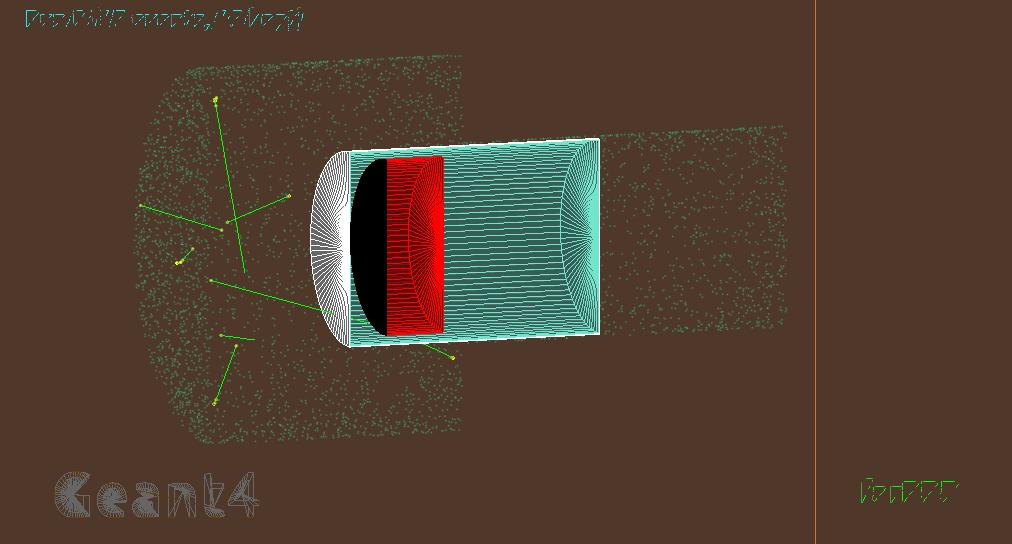
\includegraphics[width=.9\textwidth]{images/Tracks.jpg}
    \caption{Увеличенное изображение детектора в~модели.
    Красный цилиндр -- HPGe-детектор. Чёрным цветом изображён мёртвый слой -- нечувствительный объём детектора.
    Зелёные линии представляют собой треки симулируемых частиц.}\label{fig:tracks}
\end{figure}

Каждый элементарный запуск Монте-карло симуляции начинался с~рождения гамма-кванта со~случайным изотропно распределённым начальным импульсом внутри объёма условного образца.
Программа моделирует все возможные последующие взаимодействия, в~том числе рождение вторичных частиц, принимая во~внимание геометрию эксперимента.
Для частиц, попавших в~чувствительный объём детектора, регистрируется рассеянная там энергия.

Для всех энергий гамма-кванта от $0$ до $2000$~кэВ с шагом $5$~кэВ была запущена симуляция методом Монте-Карло, последовательно моделирующая $N = 10^7$ элементарных запусков.
Эффективность регистрации детектора (рис.~\ref{fig:Ey}) вычислялась как отношение зарегистрированных событий в пике к полному числу выпущенных частиц (элементарных запусков):
\begin{figure}[t]
    \centering
    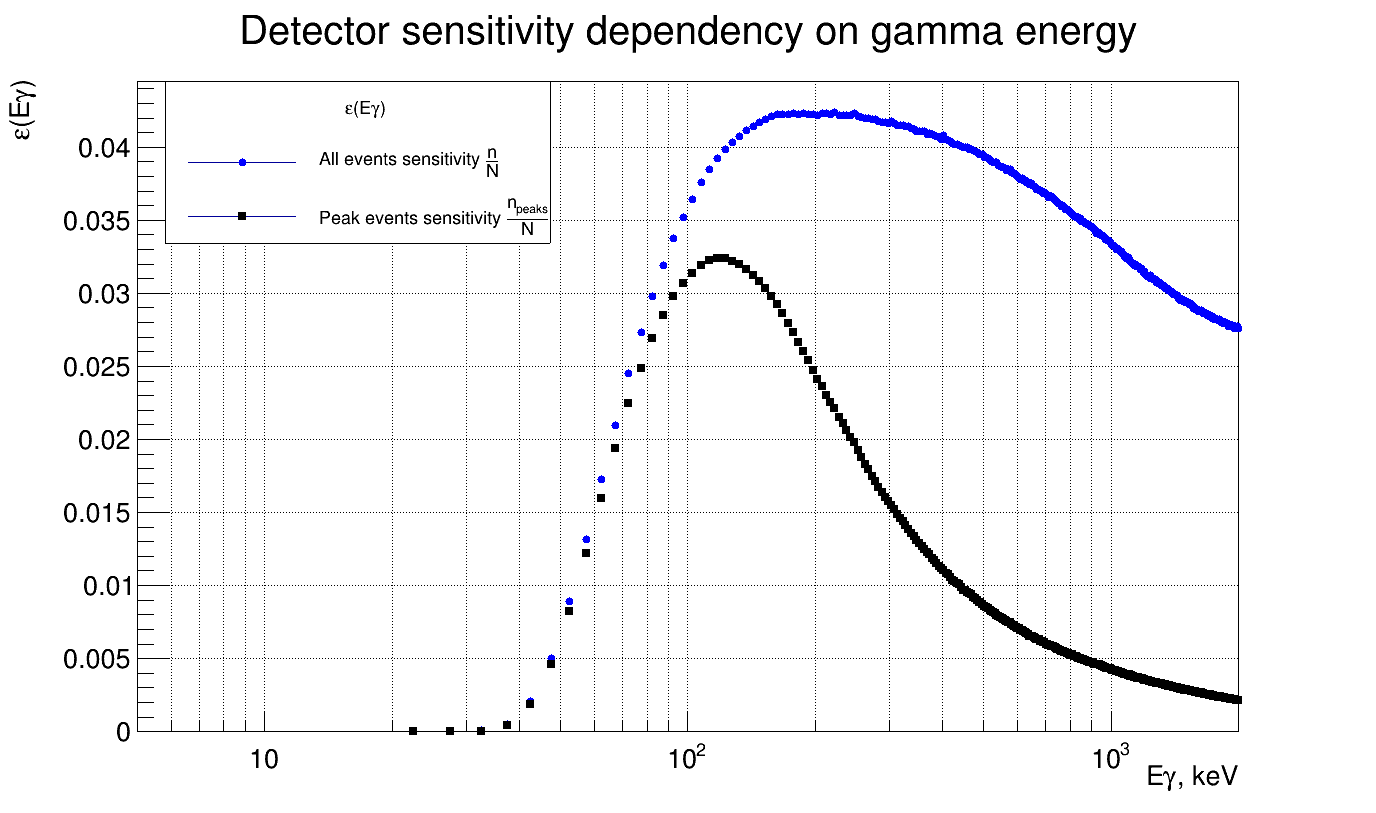
\includegraphics[width = .9\textwidth]{images/DetSens.png}
    \caption{Зависимость эффективности регистрации детектора от энергии гамма-кванта}\label{fig:Ey}
\end{figure}

Исходный код, а также подробная информация о модели доступны в репозитории на GitHub: \href{https://github.com/artem-phys/Geant4-farPPD}{github.com/artem-phys/Geant4-farPPD}

\subsection{Естественная радиоактивность сырья}
Активности изотопов для кристалла {\TmAlO} были измерены в~работе~\cite{test_bolometric_tm}.
Тем не~менее, относительно высокое содержание изотопа америция {\Am} ($A = 94 \pm 9$~Бк/кг), полученное в~данной работе, указывало на~возможный источник загрязнения данным изотопом, что требовало устранения перед проведением низкофонового эксперимента.
Измеренные на установке farPPD спектры сырья, а также вычисленная в симуляциях эффективность регистрации, позволили получить ограничение на содержание {\Am}, подтвердив радиоактивную чистоту новой партии выращенных кристаллов относительно данного изотопа.

По значениям удельной активности, предполагая скорость распада изотопов маленькой по сравнению с временем эксперимента ($T_{1/2} \gg T = 3.15 \times 10^7$~с), можно оценить число распадов конкретонго изотопа, которое будет соответствовать годовой экспозиции кристалла с~массой $8.18$~г в~установке: $N_\text{из.} \approx \frac{A \cdot m}{\lambda}$.
В~табл.~\ref{tab:sources} приведены значения определённых активностей.
\begin{table}[h!]
    \centering
    \caption{Активность нуклидов $A$ в образце и полное число распадов за год, соответствующее данной активности}\label{tab:sources}
        \begin{tabular}{rrll}
            \hline
            Цепочка &Нуклид & $A$ (Бк/кг) & Число ядер $N_{\text{из.}}$ \\
            \hline
            \hline
            \ThB    &\RaB   & 0.27               & $5.9 \times 10^{5}$  \\
                    &\ThA   & 0.22               & $1.6 \times 10^{5}$  \\\hline
            \UranB  &\RaA   & 0.45               & $2.8 \times 10^{8}$  \\
                    &\Pb    & 4                  & $3.4 \times 10^{7}$  \\\hline
            \UranA  &\UranA & 0.11               & $6.7 \times 10^{9}$  \\\hline
            --      &\K     & 0.36               & $1.7 \times 10^{14}$ \\
                    &\Co    & 0.020              & $4.0 \times 10^{4}$  \\
                    &\Am    & 0.1                & $1.6 \times 10^{7}$  \\
                    &\Cs    & 0.85               & $9.8 \times 10^{6}$  \\
        \end{tabular}
\end{table}

\subsection{Экспериментальные спектры фонового излучения}
Помимо естественного излучения радиоактивных изотопов, содержащихся в сырье для болометра, учёту подлежит также фоновое излучение внутри будущей установки.
Фоновый спектр (в отсутствие образца) был измерен также на установке farPPD в БНО.
Зарегистрированные HPGe-детектором события (рис.~\ref{fig:fon}) могут послужить разумной оценкой для моделирования распределения рождаемых фоновых гамма-квантов в симуляции будущего эксперимента по поиску аксиона:
\begin{figure}[h]
    \centering
    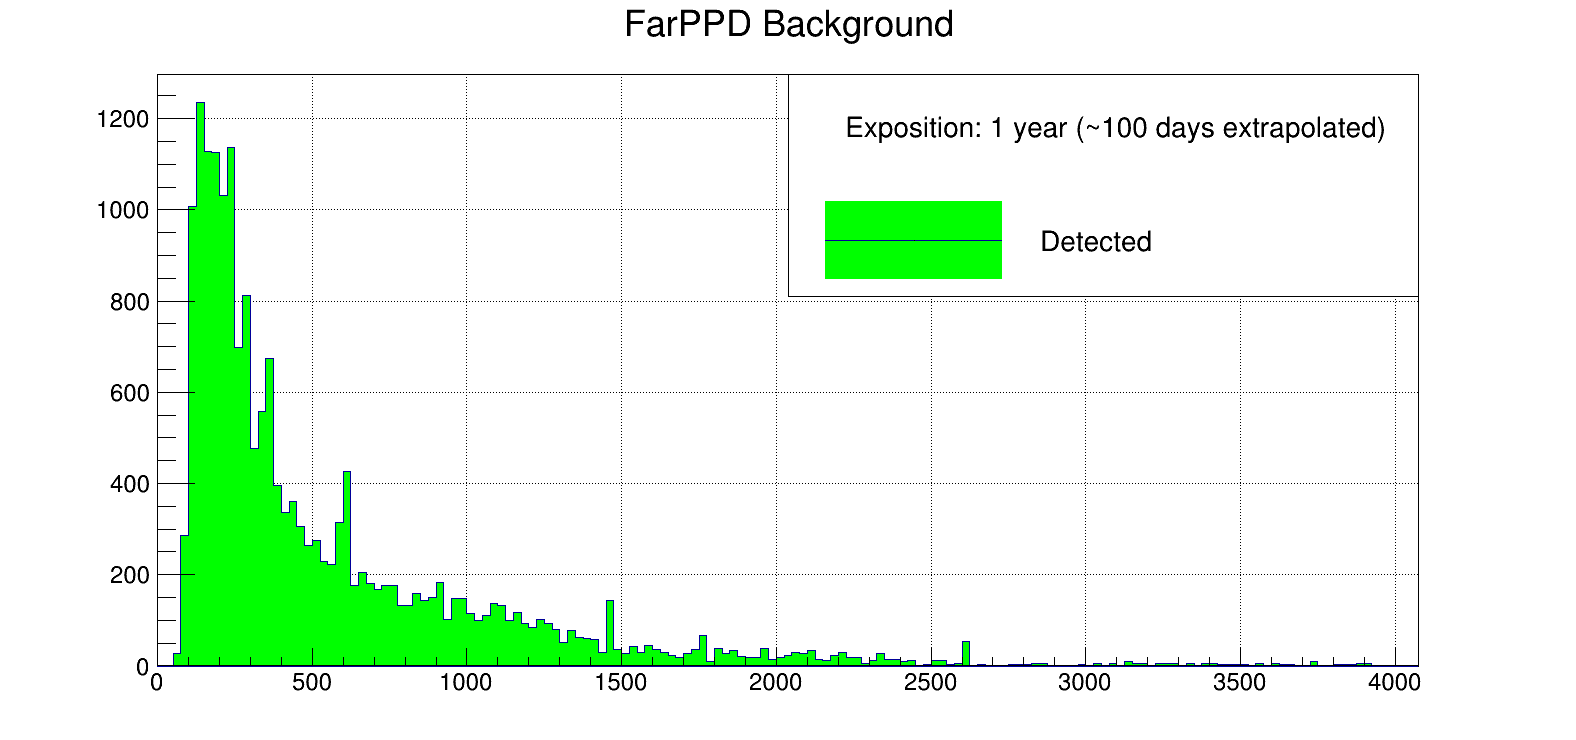
\includegraphics[width = \textwidth]{images/FarPPD_background.png}
    \caption{Фоновое излучение, зарегистрированное HPGe-детектором в отсутствие образца. Данные экстраполированы так, чтобы значения на графике соответствовали времени экспозиции 1 год}
    \label{fig:fon}
\end{figure}

События ниже энергии $50$~кэВ не записывались, так как представляют собой шумы регистрации детектора.
Ввиду того, что интересующий нас пик $8.41$~кэВ находится как раз в~указанном диапазоне, возникает необходимость сделать предположения о~спектре фонового излучения.
К счастью, отсутствие сильных характерных линий в~данном диапазоне позволяет ограничится равномерным приближением.


\pagebreak
\newpage
\section{Чувствительность будущего эксперимента по поиску аксионов}
\subsection{Моделирование эксперимента}
Предложенный низкофоновый эксперимент с криогенным тулиевым болометром был промоделирован в Geant4 методом Монте-Карло.
В качестве базы для геометрии низкофоновой защиты заимствованы размеры и материалы установки farPPD из предыдущей модели (рис.~\ref{fig:TmVis}).
Последнее связано исключительно с произвольностью выбора параметров ещё не реализованной установки.
На момент написания работы планируется размещение болометрического кристалла в криогенный криостат в MPI или в лаборатории Гран-Сассо.

Внутри вакуумной камеры по~центру расположен болометрический кристалл из~{\TmAlO} в~форме куба размером ребром $10.8$~мм (рис.~\ref{TmVisBol}).
Данный объём является чувствительным за~исключением тонкого ($d=0.01$~мм) слоя на~поверхности кристалла.
В~качестве рождаемых частиц выбраны радиоактивные изотопы, содержащиеся в~незначительном количестве в~сырье для болометра, а также гамма-кванты фонового излучения.
Вопрос определения параметров рождаемых частиц (активности изотопов и распределения по~энергиям фонового излучения) был подробно рассмотрен в~предыдущей главе.
Запуски с каждым из возможных источников были разделены: всего было проведено 9 запусков с различными нуклидами и 1 запуск для фона, включающие в себя различное число элементарных запусков, соответствующее необходимой экспозиции.
Для каждого изотопа полная эффективная экспозиция соответствует вычисленным параметрам $N_{\text{из.}}$ из таблицы~\ref{tab:sources}.
Для фонового излучения полное число симулируемых гамма-квантов и его распределение соответствует графику~\ref{fig:fon}.

В ходе элементарного запуска генерируется одна частица: либо радиоактивный изотоп, либо гамма-квант фонового излучения.
В случае, если появившийся радиоактивный изотоп не распался за время~$T_{\mathrm{stop}}$, данная частица удаляется и элементарный запуск считается завершённым.
Время~$T_{\mathrm{stop}}$ равно $1$~году и увеличивается в некоторых случаях с целью соблюдения необходимой эффективной экспозиции, если  для сокращения объёма симуляции было уменьшено число генерируемых ядер (см.~исходный код).
Для гамма-кванта таких ограничений по времени нет, и элементарный запуск обрывается с потерей энергии гамма-квантом и всеми порождёнными вторичными частицами, если такие были.

Энергия, выделившаяся в активном объёме детектора, записывается в файл.
Следует заметить, что распаду многих радиоактивных изотов соответствует одновременное рождение альфа-частиц с энергией порядка МэВ и гамма-кванта в интересующем нас кэВ-ном диапазоне.
Так как они находятся в~активном объёме детектора, им сразу регистрируется суммарная энергия данных частиц, естественно, порядка МэВ.
Возможность получить вклад от~спектра изотопов в~интересующей нас области возникает за~счёт вероятности рождения ядра в~граничном слое и улёта альфа-частицы без попадания в~детектор.
Визуализация симуляции представлена на рис.~\ref{fig:TmVis}.
\begin{figure}[t]
    \centering
    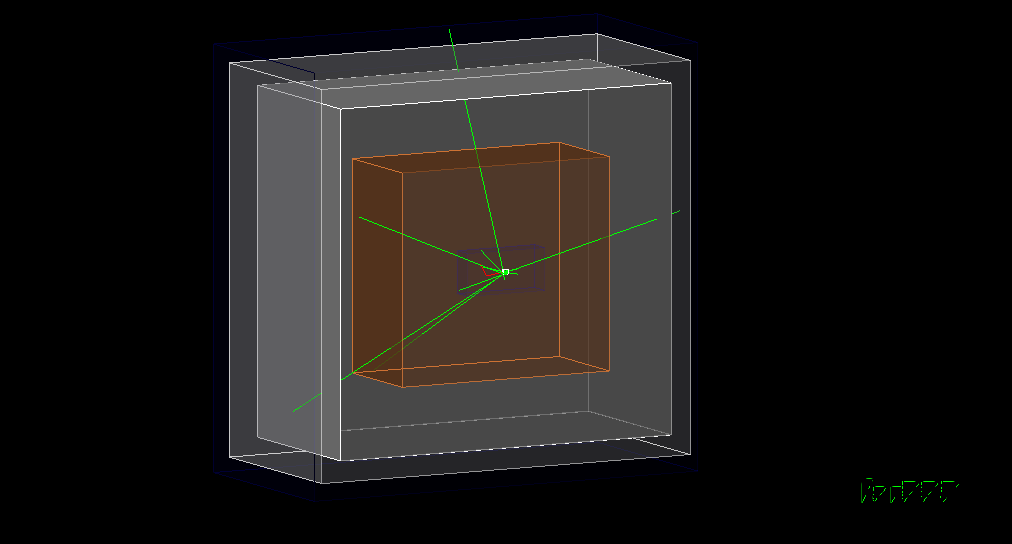
\includegraphics[width = 0.85 \textwidth]{images/TmCrystVis.png}
    \caption{Модель будущего низкофонового эксперимента по поиску аксионов в Geant4}
    \label{fig:TmVis}
\end{figure}
\begin{figure}[t]
    \centering
    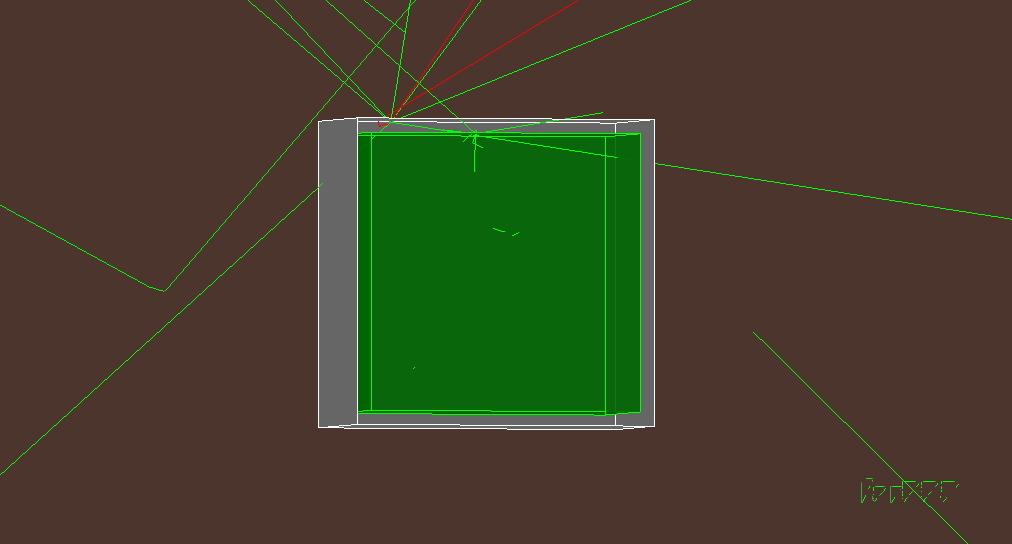
\includegraphics[width = 0.85 \textwidth]{images/Bolometer.png}
    \caption{Болометр в центре установки}
    \label{TmVisBol}
\end{figure}

Исходный код, а также подробная информация о модели доступны в репозитории на GitHub: \href{https://github.com/artem-phys/TmCryst}{github.com/artem-phys/TmCryst}

\subsection{Оценка числа возможных аксионных событий}
Результаты десяти запусков для разных источников $h_{\mathrm{source}} (E)$ были просуммированы:
\begin{equation}
    h_\mathrm{all}(E) = 
        \sum\limits_{\mathrm{source} = 0}^{10}
        f_\mathrm{source} \cdot h_\mathrm{source}(E)\, ,
\end{equation}
и полученный экспериментальный спектр симуляции $h_\mathrm{all}(E)$ для времени экспозиции $T=1$~год приведён на~рис.~\ref{hist_all}.
\begin{figure}[t]
    \centering
    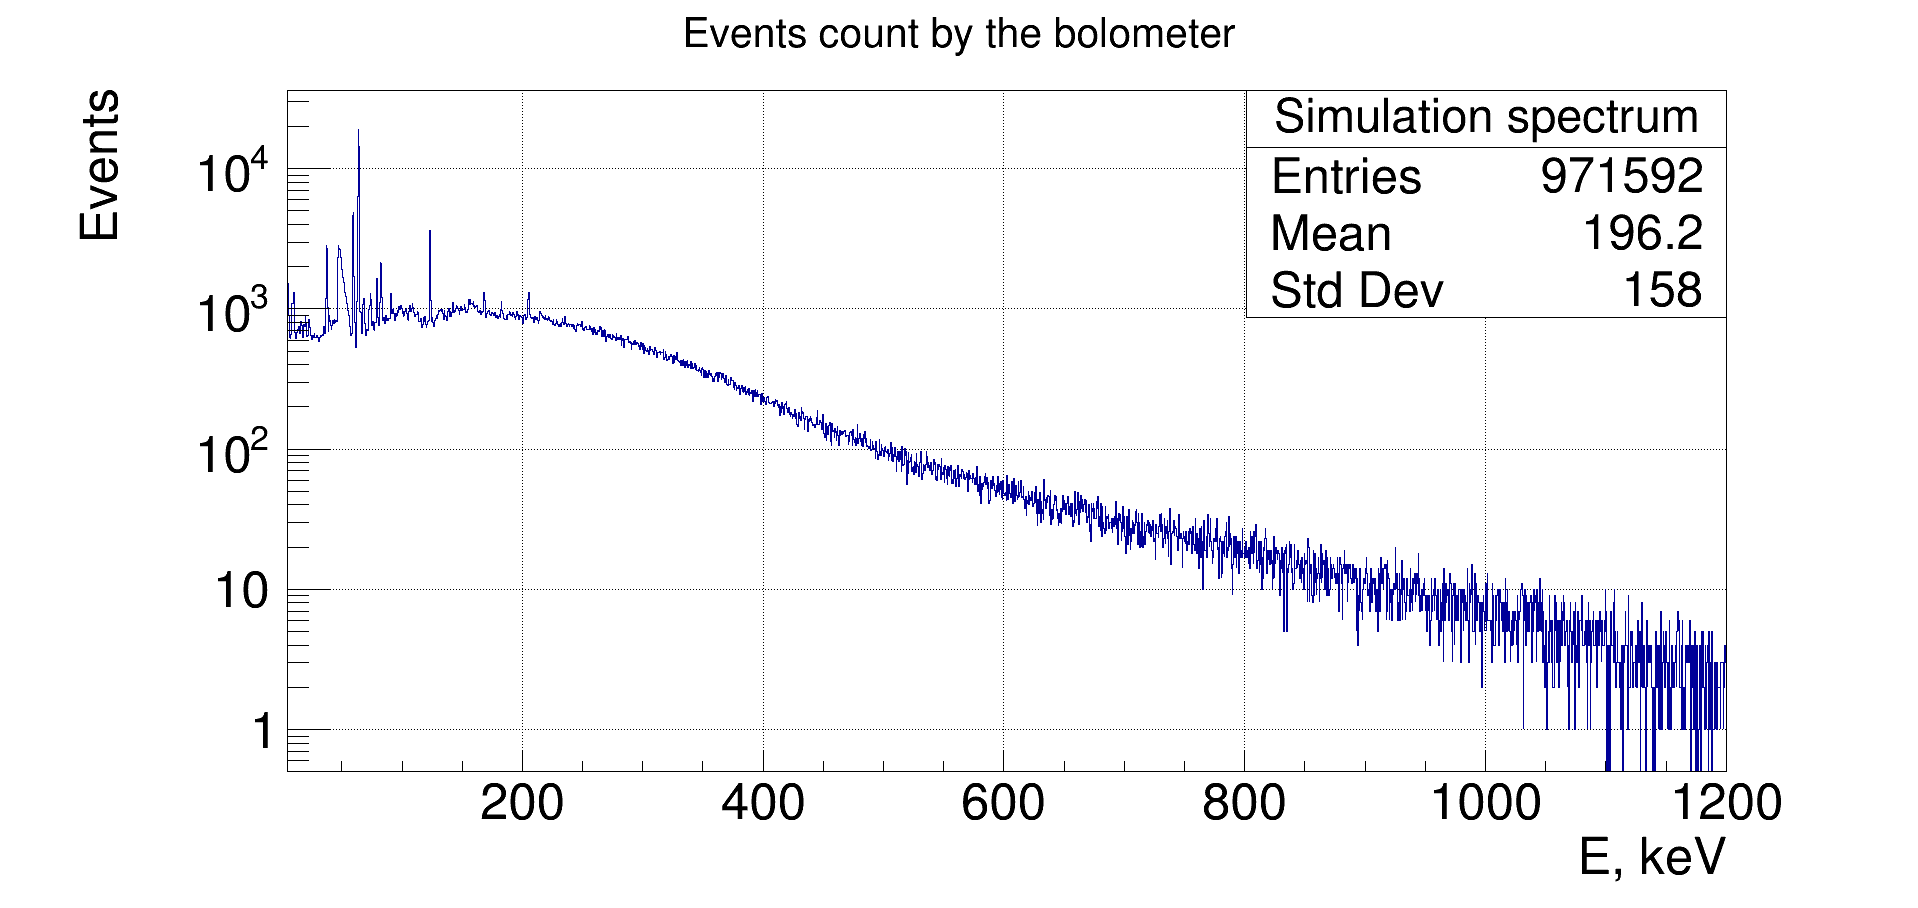
\includegraphics[width = \textwidth]{images/SpectrumTmCryst.png}
    \caption{Спектр симуляции TmCryst}\label{hist_all}
\end{figure}
\begin{figure}[t]
    \centering
    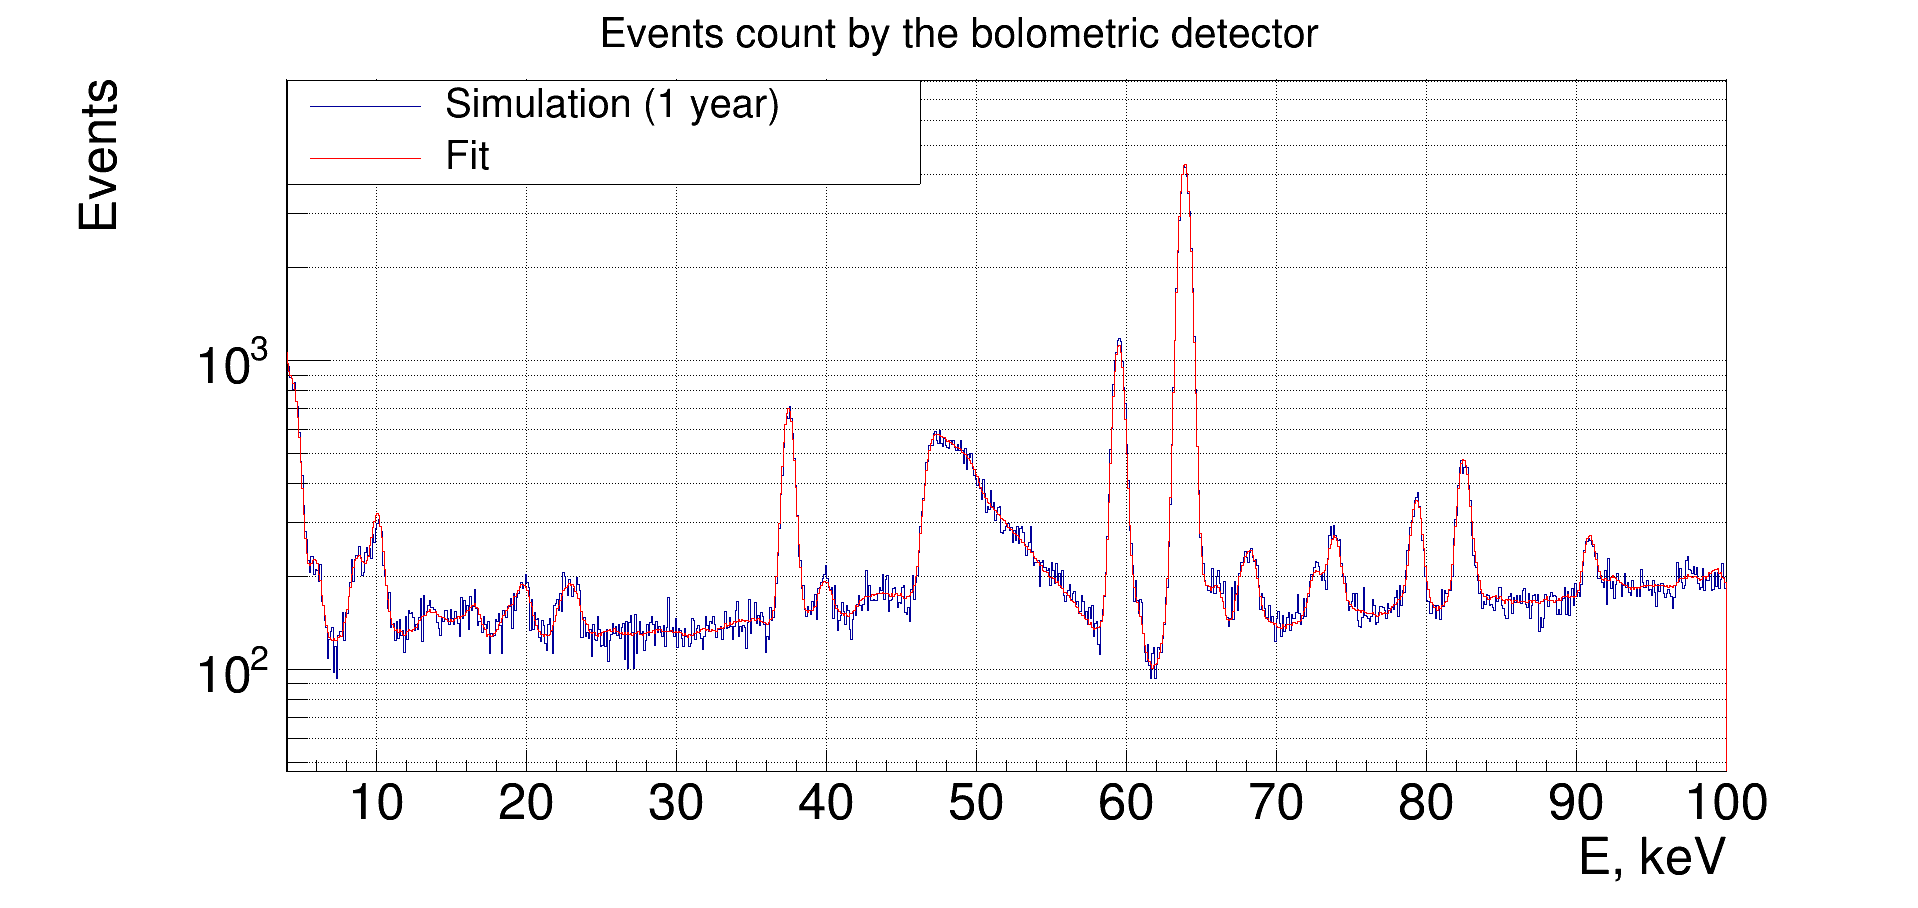
\includegraphics[width = \textwidth]{images/axion_fit.png}
    \caption{Спектр симуляции в диапазоне подгонки и результат фита}\label{AxionFit}
\end{figure}
Для получения верхнего предела на~число отсчётов в~данном пике $S_\mathrm{lim}$ использовался метод максимального правдоподобия.
Функция правдоподобия находилась в~предположении, что число отсчётов в~каждом канале гистограммы $h_{all} (E)$ имеет нормальное распределение и является линейной комбинацией Монте-Карло спектров тех же источников (но с~большей накопленной статистикой) и гауссиана, описывающего искомый аксионный пик с~энергией $E_A = 8.41$~кэВ и разрешением $\sigma = 0.38$~кэВ, взятым из~работы~\cite{test_bolometric_tm}.
Итого, подгоночная функция имеет вид:
\begin{equation}
    N(E) =
        \sum\limits_{\mathrm{source} = 0}^{10}
        f_\mathrm{source} \cdot H_\mathrm{source} (E) +
        S_A \cdot \frac{1}{\sqrt{2\pi \sigma^2} }
        \exp \left[
            - \frac{(E - {E_A})^2}{2 \sigma^2}
        \right]\, ,
\end{equation}
где $H_\mathrm{source}(E)$ -- гистограммы результатов симуляций, аналогичных $h_\mathrm{source}(E)$, но с~увеличенной в $k=10$ раз статистикой; $f_\mathrm{source}$ -- коэффициенты линейной комбинации, соответствующие доле $H_\mathrm{source}(E)$ в спектре симуляции $h_\mathrm{all} (E)$.

Общее число степеней свободы в интервале $7.7 \div 9.6$ кэВ, на котором осуществлялась подгонка, составляет $n = 32$.
Результаты фита, соответствующие минимальному значению $\chi^2 /n = \frac{116.7}{32}$ показаны на рисунке \ref{AxionFit}.
Определённое значение площади аксионного пика составило $S_A = 3 \pm 1$ событий.
Верхний предел, соответствующий $90$~\% уровню достоверности может быть найден через квантиль стандартного нормального распределения:
\begin{equation}
    S_\mathrm{lim} = S_A + u_{0.9} \cdot \Delta_{S_A} = 5\, .
\end{equation}

\subsection{Предел на константы связи}
Полное число зарегистрированных событий в пике, который можно сопоставить с аксионом, пропорционально числу ядер {\Tm} в мишени, времени измерений и эффективности регистрации детектора.
Найдём число ядер в мишени {\Tm}.
Для этого вычислим молярную массу вещества детектора:
\begin{equation}
    \mu_{\mathrm{Tm}_3 \mathrm{Al}_5 \mathrm{O}_{12}} =
        3 \cdot 168.93 + 5 \cdot 26.98 + 12 \cdot 16 =
        833.69\ \frac{\text{г}}{{\text{моль}}}\, .
\end{equation}
Каждая молекула мишени содержит $3$~ядра {\Tm}.
Подставляя массу кристалла $m = 8.18$~г, получаем:
\begin{equation}
    N_\mathrm{Tm} =
        3\nu \cdot N_A = 3 \frac{m}{\mu } N_A =
        3 \cdot \frac{8.18}{833.69} \cdot 6.022 \times {10^{23}} \approx
        1.77 \times {10^{22}}\, .
\end{equation}
Итого, полагая:
\begin{itemize}
    \item Число ядер в мишени $N_\mathrm{Tm} = 1.77 \cdot {10^{22}}$
    \item Эффективность регистрации $\varepsilon \sim 1 $, так как ядра мишени находится непосредственно внутри активного объема
    \item Время экспозиции 1 год: $T = 3.15 \cdot {10^7} c$
\end{itemize}
мы можем записать предел:
\begin{equation}
    \varepsilon \cdot T \cdot {R_A} \cdot N_{Tm} \leqslant
        {S_\mathrm{\lim }}\, .
\end{equation}

Если предположить, что $\frac{p_A}{p_\gamma} \approx 1$, то можно получить ограничения на константы связи и массу, воспользовавшись выражениями для скорости счёта ${R_A}$~\eqref{RAg1},~\eqref{RAg} и~\eqref{RAm}:
\begin{enumerate}
    \item[•] в терминах констант связи
        \begin{align}
            &\left|
                g_{A\gamma}{({g_{AN}^0 + g_{AN}^3})}
            \right| \leqslant
                2.2 \times 10^{-17} \text{ ГэВ}^{-1}\, ,\\
            &\left|
                g_{Ae}{({g_{AN}^0 + g_{AN}^3})}
            \right| \leqslant
                4.2 \times 10^{-19}\, ;\nonumber
          \end{align}
    \item[•] в терминах произведения констант связи и массы
        \begin{align}
            &\left|
                {{g_{A\gamma}}{m_A}}
            \right| \leqslant
                3.5 \times 10^{-10}\, ,\\
            &\left|
                g_{Ae} m_A
            \right| \leqslant
                7.1 \times 10^{-12} \text{ эВ}\, ;\nonumber
        \end{align}
    \item[•] в терминах массы аксиона
        \begin{equation}
            m_A \leqslant 0.12 \text{ эВ}\, .
        \end{equation}
\end{enumerate}

Приведённые верхние пределы и определяют чувствительность эксперимента.
Наличие у аксиона параметров, превышающих данные значения, позволит заметить его пик на фоне остальных зарегистрированных событий.
Сравнивая результат настоящей работы с пределами~\cite{newlimits_tm} можно заключить, что проведение низкофонового эксперимента с~криогенным тулиевым болометром поможет улучшить предыдущие ограничения приблизительно на три порядка.


\specialsection{Заключение}
Основные результаты, полученные в настоящей работе, заключаются в следующем:
\begin{enumerate}
    \item Разработана модель установки farPPD в Geant4
    \item Рассчитана $\varepsilon (E_{\gamma})$ -- эффективность регистрации HPGe-детектора, зависящая от энергии гамма-кванта, рождаемого в объёме условного образца
    \item Оценена радиоактивная чистота сырья, используемого для изготовления болометрических кристаллов {\Tm}
    \item С~использованием некоторых деталей конструкции низкофоновой защиты \textit{farPPD} разработана модель будущей установки TmCryst в~Geant4
    \item Получены экспериментальные спектры симуляции TmCryst, с~помощью которых рассчитана чувствительность будущего эксперимента по~поиску аксиона, на~три порядка превышающая существующие верхние пределы на~параметры аксиона.
\end{enumerate}

Тем самым, количественно подтверждена перспективность использования криогенного тулиевого болометра в~будущем эксперименте по~поиску аксиона --- гипотетической частицы способной пролить свет на~ряд нерешённных вопросов современной физики.
Разработанные подходы и программное обеспечение могут быть полезны при подготовке, проведении и анализе данных реального эксперимента.

Работа выполнена при поддержке Российского фонда фундаментальных исследований, проект №~19-02-00097.


\pagebreak
\printbibliography[title={Источники}]{}

\end{document}